\documentclass{article}
\usepackage[a4paper, margin=1in]{geometry}
\usepackage[utf8]{inputenc}
\usepackage[T1]{fontenc}
\usepackage{lmodern}
\usepackage{amsmath, amssymb, graphicx, hyperref}
\graphicspath{{../figures/}}
\usepackage{bookmark}
\usepackage[framed,numbered]{matlab-prettifier}
\usepackage{xcolor}
\usepackage{listings}
\pagenumbering{gobble}

\geometry{a4paper, margin=1in}

% MATLAB code style
\lstset{
  style      = Matlab-editor,
  basicstyle = \mlttfamily,
  breaklines = true
}

\title{\textbf{Practical - 2}}
\author{}
\date{October 3, 2026}

\begin{document}
\maketitle

\noindent
\textbf{\large{Aim:}} To plot the solution family of a second-order differential equation.

\vspace{1em}
\noindent
\textbf{\large{MATLAB Code:}}

\begin{lstlisting}
clc; clear  all; close all;

syms y(x)

eqn = diff(y,2) + y == 0;
ySol = dsolve(eqn);

disp('General solution:')
disp(ySol)

hold on
fplot(subs(ySol, {'C1', 'C2'},{1, 0}), [0 2*pi], 'LineWidth',1.5)
fplot(subs(ySol, {'C1', 'C2'},{2, 0}), [0 2*pi], 'LineWidth',1.5)
fplot(subs(ySol, {'C1', 'C2'},{1, 1}), [0 2*pi], 'LineWidth',1.5)
fplot(subs(ySol, {'C1', 'C2'},{1, -1}), [0 2*pi], 'LineWidth',1.5)

grid on
xlabel('x')
ylabel('y(x)')
title('Family of Solutions of d^2y/dx^2 + y = 0')
legend('C1=1, C2=0', 'C1=2, C2=0', ...
    'C1=1, C2=1', 'C1=1, C2=-1', ...
    'Location','best')
hold off

\end{lstlisting}

\vspace{1em}
\noindent
\textbf{\large{Output:}}

\begin{flushleft}
\tiny{General solution:}
\end{flushleft}

\begin{flushleft}
    $C_1 \,\cos \left(x\right)-C_2 \,\sin \left(x\right)$
\end{flushleft}

\newpage
\vspace{0.5em}
\begin{figure}[htbp]
    \centering
    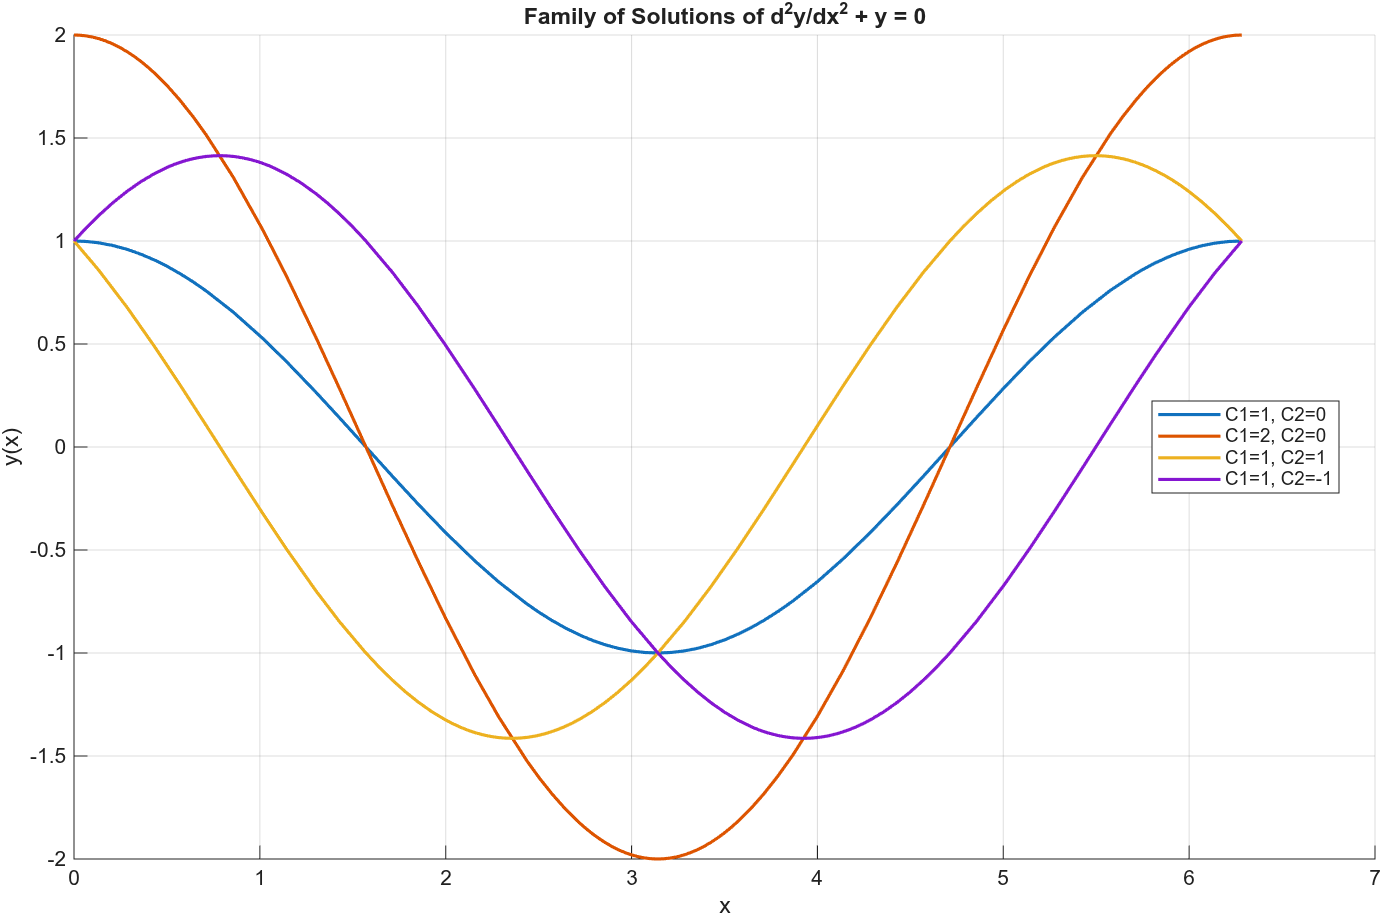
\includegraphics[width=0.7\textwidth]{Figure2.png}
\end{figure}

\vspace{1em}
\noindent
\fbox{%
    \begin{tabular}{@{}l@{}}
        \textbf{\large{NOTE:}} \\
        \textbf{subs(...)} Substitutes chosen values for the arbitrary constants to create individual solutions. \\
        \textbf{fplot(..., [0 2*pi])} Plots each curve from $x = 0$ to $x = 2\pi$.
    \end{tabular}%
}

\end{document}
